\documentclass[12pt, a4paper]{article}

\usepackage{amsmath,amsthm,amssymb}
\usepackage{mathtext}
\usepackage[T1,T2A]{fontenc}
\usepackage[utf8]{inputenc}
\usepackage[english,russian]{babel}

\usepackage{graphicx}
\graphicspath{{images/}}

\title{Plato Solids}
\author{Антипов Дмитрий\\19ИТ-МО}
\date{2023}

\begin{document}

\maketitle

Постановка задачи:
\begin{list}{}{}
	\item Построение и отрисовка платоновых тел в среде OpenGL.
\end{list}

\hfill \break

Описание:
\begin{list}{}{}
	\item При запуске проекта создаются 5 тел - по одному каждого типа, им даётся случайные вектора движения (трансляции) и поворота (по 3 осям, используются описание поворота как произведения 3 матриц поворота относительно каждой из осей).
	\item Тела отталкиваются от границ сцены, а так же при столкновении друг с другом.
	\item При создании объекта, можно указать начальное положение и длину ребра фигуры.
	\item Объект в себе содержит координату отрисовки фигуры и саму фигуру.
	\item Фигуры строются таким образом, что все ребра имеют одинаковую длину.
\end{list}

\break

Проект написан в среде Visual Studio Code с использованием языка программирования Python v.3.11.

Порядок разработки проекта:
\begin{list}{}{}
	\item Создаётся сущность App - приложение, которая будет отвечать за отрисовку окна и выступать менеджером отрисовки фигур.
	\item Создаётся сущность Object - объект, который содержит информацию о позиции в пространстве, векторе движения и поворота. Внутри него содержится фигура, которую мы и рисуем на экране. При совершении трансформаций Переноса и Поворота изменяется именно объект, а не фигура внутри.
	\item Создаётся сущность Shape3D - объёмная фигура, которую мы будем отрисовывать. Содержит методы и поля, единые для всех фигур.
	\item Создаётся сущность Composer3D - менеджер создания трёхмерных фигур. В качестве задания выбраны (в скобках кол-во граней):
	\begin{list}{-}{}
		\item Куб(6)
		\item Тетраэдр(4)
		\item Октаэдра(8)
		\item Икосаэдр(20)
		\item Додекаэдр(12)
	\end{list}
	\item По аналогии с Shape3D и Composer3D создаются сущности Shape2D и Composer2D, которые используются для двумерных фигур.
	\item Создаются сущности Matrix и Vertex (Матрица и Вершина соответственно), которые используются для математических операций.
	\item Используются функции из файла console - для форматирования вывода
	\item Используются константы из файла utils - для сохранения значений освещения сцены, позиции камеры и палитры цветов фигур.
\end{list}

Проект состоит из:
\begin{list}{-}{}
	\item console.py - Функции для форматирования вывода в консоль;
	\item utils.py - Подключение необходимых графических библиотек и описание констант;
	\item matrix.py - Функции для работы с векторами и матрицами;
	\item vertex.py - Функции для работы с вершинами фигур;
	\item shape2d.py - Функции для работы с двумерными фигурами;
	\item composer2d.py - Функции описания различных двумерных фигур;
	\item shape3d.py - Функции для работы с трёхмерными фигурами;
	\item composer3d.py - Функции описания различных трёхмерных фигур;
	\item object.py - Функции для работы с объектами;
	\item app.py - Функции для работы с главным приложением;
	\item main.py - Главная функция запуска проекта.
\end{list}

\hfill \break

Для реализации проекта были использованы библиотеки:
\begin{list}{-}{}
	\item PyOpenGL - Реализация графической библиотеки OpenGL на языке Python;
	\item PyGame - Библиотека для создания окна, где будет отображаться графика.
\end{list}

\hfill \break

В файле source\_code.pdf можно ознакомиться с исходным кодом проекта.

\hfill \break

Для запуска проекта
\begin{list}{}{}
	\item Перейдите в заглавную папку проекта "Plato Solids" и запустите файл программы "Plato Solids.exe"
	\item Можно запустить непосредственно код проекта, запустив файл "run.bat", при этом будут установлены все библиотеки, необходимые программе.
	ПРИМ. : Требуется Python v3 и старше.
	\item Кроме этого можно вызвать командную строку и выполнить команду "python ./src/main.py"
\end{list}

\hfill \break

\begin{figure}[h]
	\centering
	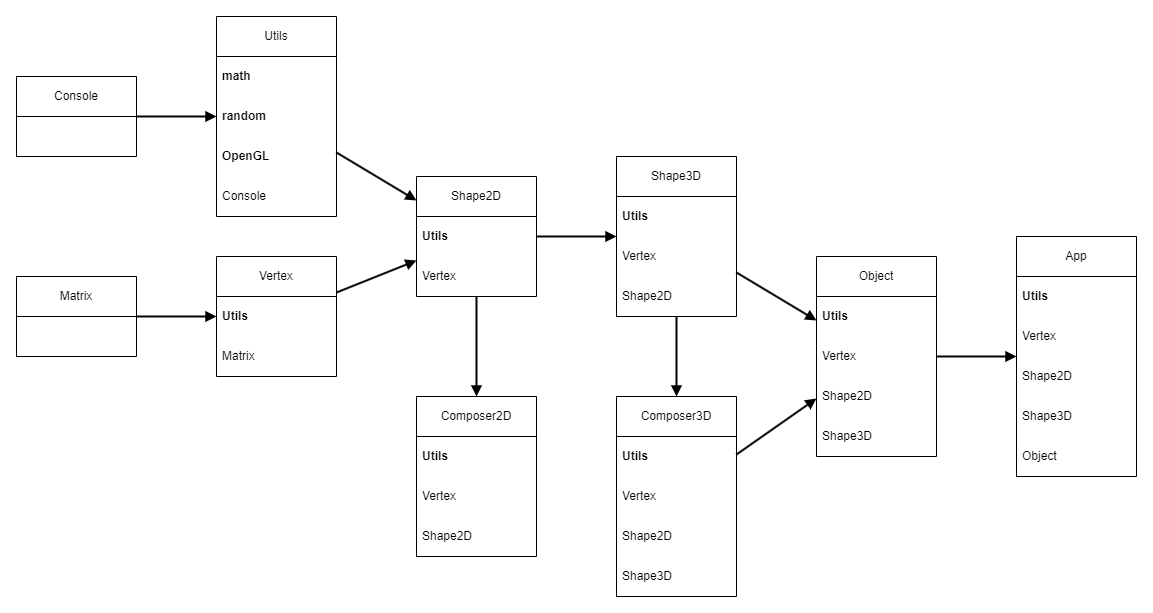
\includegraphics[scale=.35]{structure}
	\caption{структура проекта}
	\label{fig:mesh1}
\end{figure}

\begin{figure}[h]
	\centering
	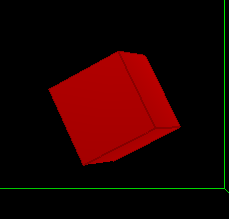
\includegraphics[scale=1.25]{cube}
	\caption{Отрисовка Куба}
	\label{fig:mesh1}
\end{figure}

\begin{figure}[h]
	\centering
	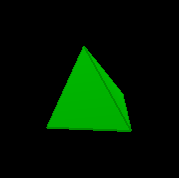
\includegraphics[scale=1.75]{pyramid}
	\caption{Отрисовка Тетраэдра}
	\label{fig:mesh1}
\end{figure}

\begin{figure}[h]
	\centering
	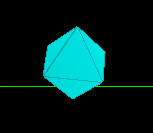
\includegraphics[scale=2]{oct}
	\caption{Отрисовка Октаэдра}
	\label{fig:mesh1}
\end{figure}

\begin{figure}[h]
	\centering
	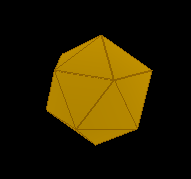
\includegraphics[scale=1.5]{ico}
	\caption{Отрисовка Икосаэдра}
	\label{fig:mesh1}
\end{figure}

\begin{figure}[h]
	\centering
	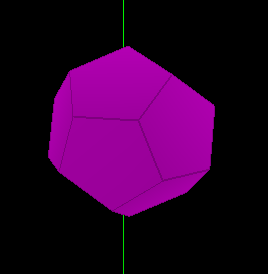
\includegraphics[scale=1.1]{dod}
	\caption{Отрисовка Додекаэдра}
	\label{fig:mesh1}
\end{figure}

\begin{figure}[h]
	\centering
	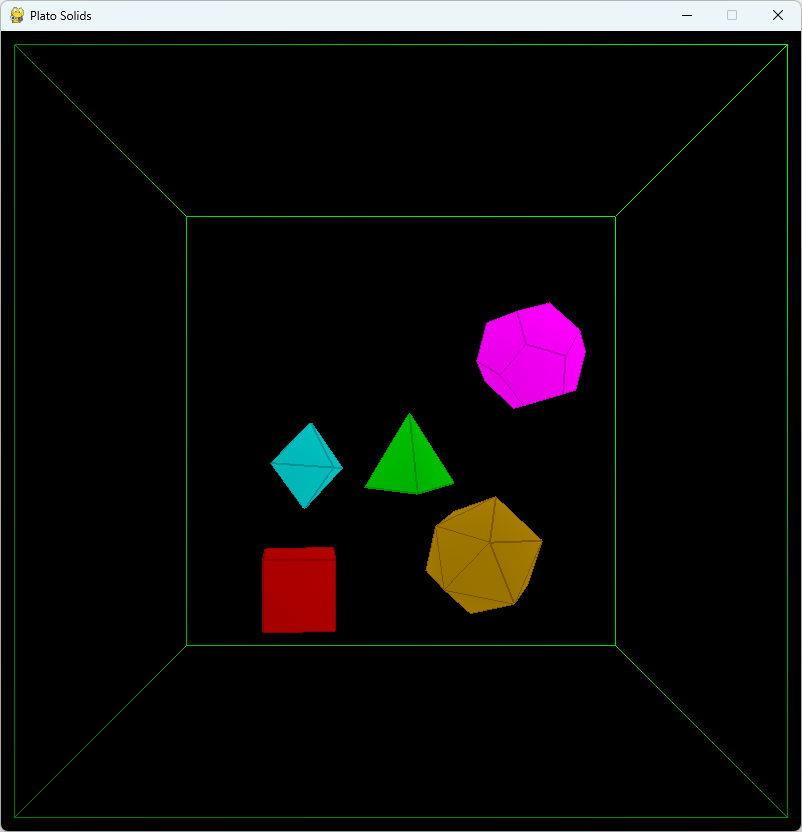
\includegraphics[scale=.6]{all}
	\caption{Окно проекта - отрисовка всех фигур}
	\label{fig:mesh1}
\end{figure}

\end{document}